\subsection{CAF benchmark}\label{subsec:caf}

This subsection reports the parallel scaling analysis of Euler 1D test programs (with and without FOODIE) being parallelized by means of CoArrays Fortran (CAF) model. This parallel model is based on the concept of \emph{coarray} introduced into the Fortran 2008 standard: the array syntax is extended introducing the so called \emph{codimension} that is a new arrays indexing. Essentially, a CAF enabled code is designed to be replicated a certain number of times and all copies, conventionally named \emph{images}, are executed asynchronously. Each image has its own set of data (memory) and the codimension indexes are used to access to the (remote) memory of the other images. The CAF approach allows the implementation of Partitioned Global Address Space (PGAS) model following the SPMD (single program, multiple data) parallelization paradigm. The programmer must take care of defining the coarray variables and of synchronizing the images when necessary. This approach requires the refactoring of legacy serial codes, but it allows the exploitation of both shared and distributed memory architectures. Moreover, it is a standard feature of Fortran (2008), thus it is not chained to any particular compiler vendors extension.

\begin{figure}[!ht]
  \centering
  \begin{subfigure}[b]{0.80\textwidth}
    \centering
    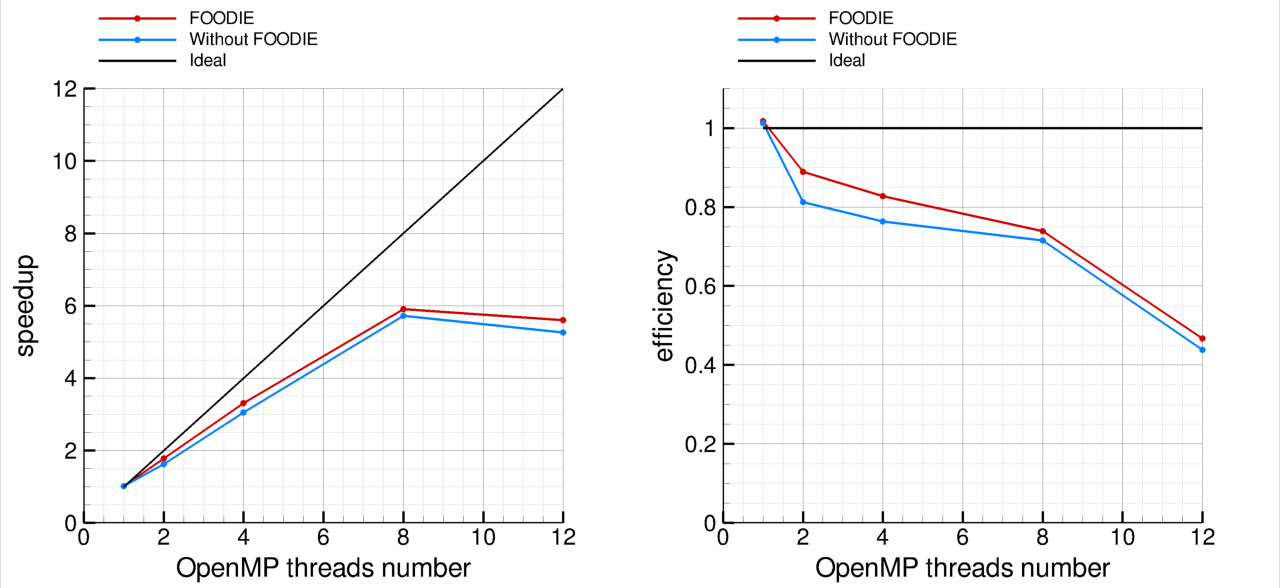
\includegraphics[width=1.00\textwidth]{caf_benchmark/euler-1D-caf/strong-scaling-comparison.png}
    \caption{Strong scaling, number of cells 240000}\label{fig:strong-scaling-caf}
  \end{subfigure}\\
  \begin{subfigure}[b]{0.80\textwidth}
    \centering
    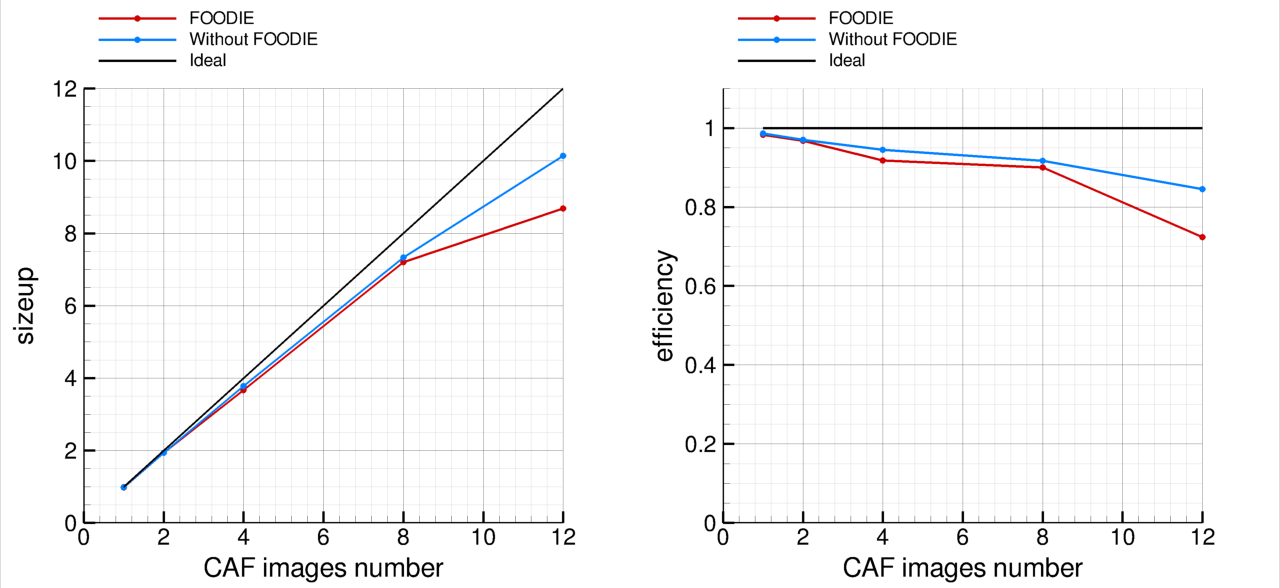
\includegraphics[width=1.00\textwidth]{caf_benchmark/euler-1D-caf/weak-scaling-comparison.png}
    \caption{Weak scaling, minimum number of cells 24000}\label{fig:weak-scaling-caf}
  \end{subfigure}\\
  \caption{Scaling efficiency with CAF programming model}\label{fig:scaling-caf}
\end{figure}

The benchmarks shows in this section have been done on a \emph{dual Intel(R) Xeon(R) CPU X5650} exacores workstation for a total of 12 physical cores, coupled with 24GB of RAM. In order to perform an accurate analysis 4 different codes have considered:

\begin{itemize}
  \item FOODIE-aware codes:
    \begin{itemize}
      \item serial code;
      \item CAF-enabled code;
      \end{itemize}
  \item procedural codes without using FOODIE library:
    \begin{itemize}
      \item serial code;
      \item CAF-enabled code;
      \end{itemize}
  \end{itemize}

These codes (see \ref{subsec:euler-1D-CAF-API} for the implementation details) have been compiled by means of the GNU gfortran compiler v5.2.0 coupled with OpenCoarrays v1.1.0\footnote{OpenCoarrays is an open-source software project for developing, porting and tuning transport layers that support coarray Fortran (CAF) compilers, see \cite{opencoarrays}.}.

The Euler conservation laws are integrated for 30 time steps by means of the TVD RK(5,4) solver: the measured CPU time used for computing the scaling efficiencies is the average of the 30 integrations, thus representing the mean CPU time for computing one time step integration.

For the strong scaling, the benchmark has been conducted with 240000 finite volumes. Figure \ref{fig:strong-scaling-caf} summarizes the strong scaling analysis: it shows that FOODIE-based code scales similarly to the baseline code without FOODIE.

For the weak scaling the minimum size is 24000 finite volumes and the size is scaled linearly with the CAF images, thus $N_{12} = 288000$ cells. Figure \ref{fig:weak-scaling-caf} summarizes the weak scaling analysis and it essentially confirms that FOODIE-based code scales similarly to the baseline code without FOODIE.

Both strong and weak scaling analysis point out that for the computing architecture considered the parallel scaling is reasonable up to 12 cores, the efficiency being always satisfactory.

To complete the comparison, the absolute CPU-time consumed by the two families of codes (with and without FOODIE) must be considered. Table \ref{tab:caf-results} summarizes the benchmarks results. As shown, procedural and FOODIE-aware codes consume a very similar CPU-time for both the strong and the weak benchmarks. The same results are shown in figure \ref{fig:cpu-time-caf}. These results prove that the abstraction of FOODIE environment does not degrade the computational efficiency.

\begin{table}[!ht]
  \centering
  \caption{caf benchmarks results\label{tab:caf-results}}
  \begin{subtable}[b]{0.80\textwidth}
    \centering
    \caption{Strong benchmarks, number of cells 240000\label{tab:caf-results-strong}}
    \resizebox{1.00\textwidth}{!}{%
    \begin{tabular}{ccccc}
      {\sc Number of caf threads} & \multicolumn{4}{c}{\sc CPU time for 1 time step integration}              \\
      \hline
                                     & FOODIE serial & FOODIE parallel & procedural serial & procedural parallel \\
      \cmidrule{2-5}
      1                              & 3.2970        & 3.3297          & 3.0049            & 3.0563              \\
      2                              & /             & 1.6536          & /                 & 1.5686              \\
      4                              & /             & 0.8515          & /                 & 1.8116              \\
      8                              & /             & 0.4296          & /                 & 0.4130              \\
      12                             & /             & 0.3094          & /                 & 0.2839              \\
      \hline
    \end{tabular}}
  \end{subtable}\\
  \begin{subtable}[b]{0.80\textwidth}
    \centering
    \caption{Weak benchmarks, minimum number of cells 24000\label{tab:caf-results-weak}}
    \resizebox{1.00\textwidth}{!}{%
    \begin{tabular}{cccccc}
      {\sc Number of caf threads} & {\sc Number of Cells} & \multicolumn{4}{c}{\sc CPU time for 1 time step integration} \\
      \hline
                                     &                       & FOODIE serial & FOODIE parallel & procedural serial & procedural parallel \\
      \cmidrule{3-6}
      1                              & 24000                 & 0.3105        & 0.3159          & 0.3089            & 0.3133              \\
      2                              & 48000                 & /             & 0.3209          & /                 & 0.3185              \\
      4                              & 96000                 & /             & 0.3384          & /                 & 0.3269              \\
      8                              & 192000                & /             & 0.3449          & /                 & 0.3369              \\
      12                             & 288000                & /             & 0.4291          & /                 & 0.3657              \\
      \hline
    \end{tabular}}
  \end{subtable}
\end{table}

\begin{figure}[!ht]
  \centering
  \begin{subfigure}[b]{0.40\textwidth}
    \centering
    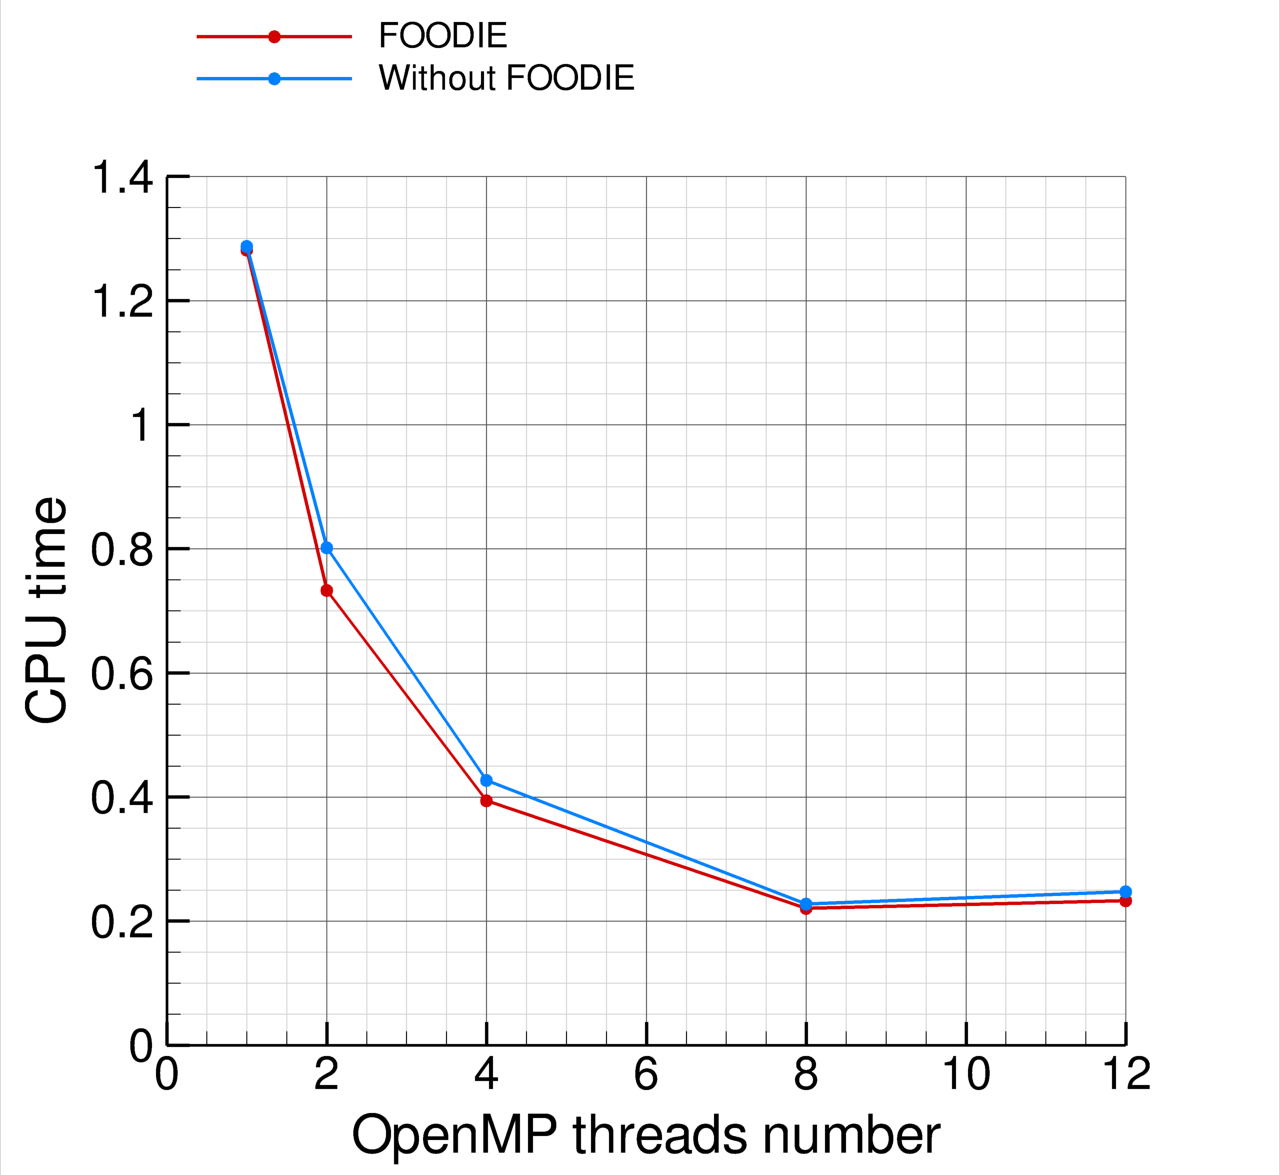
\includegraphics[width=1.00\textwidth]{caf_benchmark/euler-1D-caf/strong-cpu-time-comparison.png}
    \caption{Strong benchmark, number of cells 240000}\label{fig:strong-cpu-time-caf}
  \end{subfigure}\quad%
  \begin{subfigure}[b]{0.40\textwidth}
    \centering
    \includegraphics[width=1.00\textwidth]{caf_benchmark/euler-1D-caf/weak-cpu-time-comparison.png}
    \caption{Weak benchmark, minimum number of cells 24000}\label{fig:weak-cpu-time-caf}
  \end{subfigure}\\
  \caption{CPU time consumed with caf programming model}\label{fig:cpu-time-caf}
\end{figure}

